%卒業論文概要テンプレート ver. 1.0

\documentclass[uplatex,twocolumn,dvipdfmx]{jsarticle}
\usepackage[top=22mm,bottom=22mm,left=20mm,right=20mm]{geometry}
\setlength{\columnsep}{15mm}
\usepackage[T1]{fontenc}
\usepackage{txfonts}
\usepackage{wrapfig}
\usepackage[expert,deluxe]{otf}
\usepackage[dvipdfmx,hiresbb]{graphicx}
\usepackage[dvipdfmx]{hyperref}
\usepackage{pxjahyper}
\usepackage{secdot}

\makeatletter
\renewcommand{\section}{%
  \@startsection{section}{1}{\z@}%
  {0.6\Cvs}{0.4\Cvs}%
  {\normalfont\normalsize\raggedright}}
\renewcommand{\subsection}{\@startsection{subsection}{2}{\z@}%
  {\z@}{\z@}%
  {\normalfont\normalsize}}
\renewcommand{\subsubsection}{\@startsection{subsubsection}{3}{\z@}%
  {\z@}{\z@}%
  {\normalfont\normalsize}}
\makeatother
%ここから上を編集する必要はない.





%タイトルと学生番号,名前だけ編集すること
\title{\vspace{-5mm}\fontsize{14pt}{0pt}\selectfont GitHub上のソフトウェア開発のためのフロー推薦手法}
\author{\normalsize プロジェクトマネジメントコース・ソフトウェア開発管理グループ 矢吹研究室 1242132 若月 純}
\date{}
\pagestyle{empty}
\begin{document}
\fontsize{10.5pt}{\baselineskip}\selectfont
\maketitle





%以下が本文
\section{序論}
ソフトウェア開発では,複数のメンバが同時に開発を行うため,様々な問題が発生する.問題を解決するため,バージョン管理システムを用いる.バージョン管理システムとは,変更履歴を管理するシステムのことである\cite{ikeda2014}.

バージョン管理システムを提供するサービスに,GitHubがある.GitHubは,バージョン管理システムに加え,開発を補助する機能を提供するサービスである.

GitHubを使用する手順を開発フローと呼ぶ.開発フローは,13種類あり,それぞれメリットとデメリットがある.しかし,選択する基準は定められていないため,状況にあった開発フローを選択するのは難しい.そのため,適切でない開発フローを選択し,開発に悪影響を与える危険がある.

そこで,本研究では,適切な開発フローを選択できるようにするための基準を求める.



\section{目的}

GitHubを用いたソフトウェア開発プロジェクトの性質において,適切な開発フローを選択できるようにするための基準を求める.

\section{手法}

初めに,GitHub上のプロジェクトから,開発フローの採用に関わると思われるの指標を調査する.

次に,採用されている開発フローを調査する.開発フローの正解データは,人手で作成する.

最後に,プロジェクトに関する上述の指標から,開発フローを決めるための決定木の作成を試みる.


\section{結果}

% 大文字のHを使用することで好きな位置に図を配置
\begin{figure}
%\includegraphics[width=図の幅,clip]{ファイル名}\label{参照用ラベル}
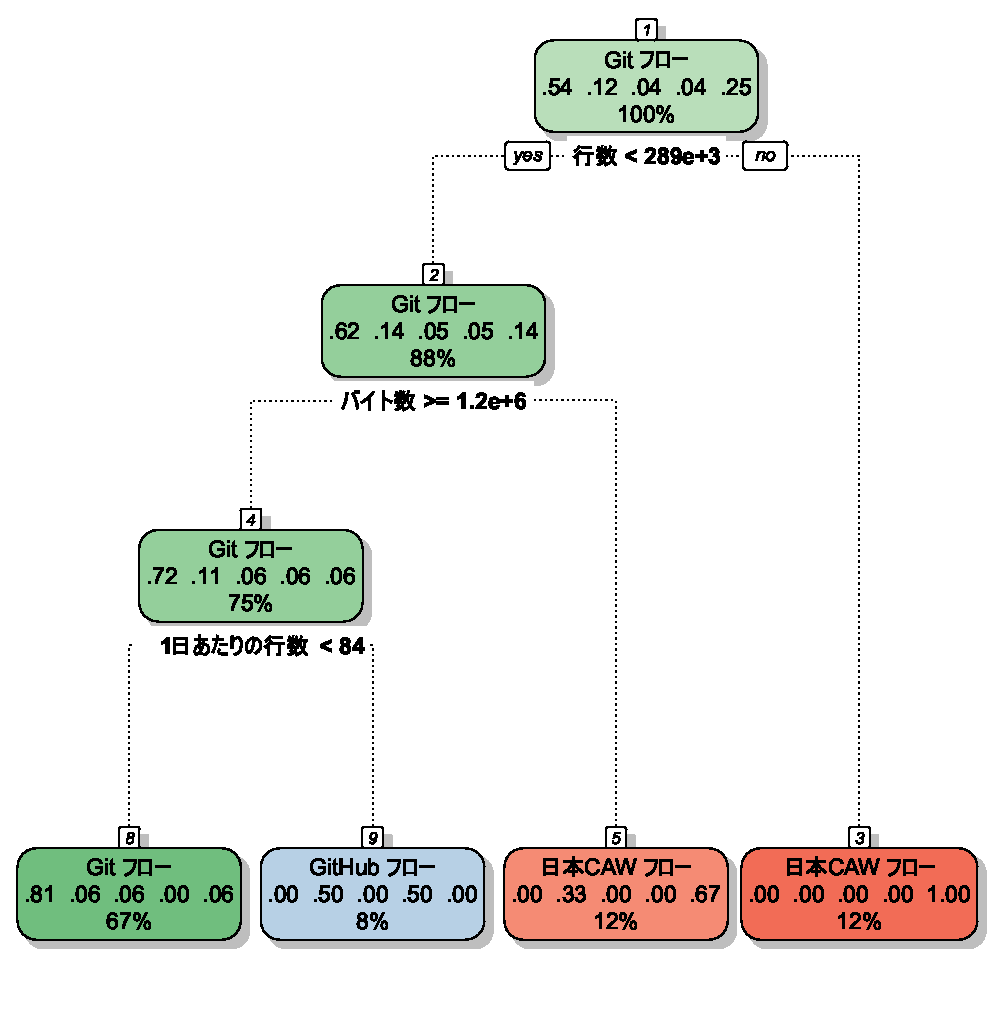
\includegraphics[width=8cm,clip]{decisiontree.eps}
\caption{プロジェクトの性質により選択される開発フローの違い}\label{決定木}
\end{figure}


決定木分析結果が,図1である.

図1より,行数,バイト数,1日あたりの行数で,選択されている開発フローを割り出せられる.

開発フローのわかっているプロジェクトを使って作成された開発フローの決定木が,開発フローが未知のプロジェクトの開発フローを予測できるかどうかを試したところ,精度は平均$38$\%(信頼区間は$33\sim 42$\%),再現率は平均$46$\%(信頼区間は$41\sim 51$\%)だった.



\section{考察}

1日あたりの行数といった,時系列データにより分類されていることが分かった.ここから,他の時系列データを調査することで,より精度と再現率をあげられると考えられる.

\section{結論}

本研究では,決定木を用いた,開発フローを推薦する手法を提案した.
現状では,精度と再現率が高いとは言えないが,このような手法を発展させることによって,GitHubの経験が少ないチームでの開発でも,最適なフローを決定できるようになることが期待される.

\bibliographystyle{junsrt}
\bibliography{biblio}%「biblio.bib」というファイルが必要.

\end{document}
